\documentclass[11pt]{article}

\usepackage{amsmath}
\usepackage{textcomp}
\usepackage[top=0.8in, bottom=0.8in, left=0.8in, right=0.8in]{geometry}
\usepackage{graphicx}
\usepackage{subcaption}
\usepackage{hyperref}
\usepackage[english]{babel}

\graphicspath{ {report_images/} }
% Add other packages here %

\catcode`\_=\active
\protected\def_#1_{\textit{#1}}

% Put your group number and names in the author field %
\title{\bf Excercise 1.\\ Implementing a first Application in RePast: A Rabbits Grass Simulation.}
\author{Group \textnumero 25: Boris Goullet, Julien Grondier}

\begin{document}
\maketitle

\section{Implementation}

\subsection{Assumptions}
% Describe the assumptions of your world model and implementation (e.g. is the grass amount bounded in each cell) %

We assumed that there could only exist one ``unit'' of grass per tile.
\\Default parameters:
\begin{itemize}
\setlength\itemsep{0pt}
\item Size of space is 20x20, as specified in assignment
\item Number of rabbits at start is 20
\item Cost of spawning a new rabbit is 20 energy ``units''
\item Number of new grass tiles spawning per step is 10
\item Energy ``units'' a rabbit receives when eating a grass tile is 7
\item Starting energy for rabbits (both newly spawned and ones there at the start) is 7
\end{itemize}

\subsection{Implementation Remarks}
% Provide important details about your implementation, such as handling of boundary conditions %
For most points, we followed the RePast tutorial given by the assignment, as such, the code is not that different.\\

Every step, _grassGrowthRate_ barren ground tiles have grass grow on them: a list of all barren tiles is constructed, then _grassGrowthRate_ tiles are randomly picked from this list, and are changed to have grass. If all tiles have grass (respectively not enough tiles are barren), then no new grass tiles are created (respectively all barren tiles receive grass).

When a new rabbit is born, the parent loses exactly _birthCost_ energy, the newborn starts with exactly _startingEnergy_ and is at a random free tile. If no tiles are free, the parent still loses the energy, but no new agent is added. A similar algorithm to the one for the grass tile placement is used to determine where/if to place the new rabbit.

When a rabbit wants to move (i.e. every step), it chooses a random cardinal direction. Then, if the tile in the chosen direction already contains a rabbit, the rabbit attempting to move instead does not move for this step, but still loses one energy ``unit''.


\section{Results}
% In this section, you study and describe how different variables (e.g. birth threshold, grass growth rate etc.) or combinations of variables influence the results. Different experiments with diffrent settings are described below with your observations and analysis
We ran simulations with differents values changed. Some results were rather evident (e.g. setting _grassGrowthRate_ or _grassEnergy_ to very low values means most, if not all, rabbits will die from hunger; or having a too large world size compared to the _grassGrowthRate_ means the rabbits will not find the grass and die of hunger, since their random movement means finding grass is pure luck).

See Figure \ref{fig:default} for a typical simulation run with the default parameters.

\begin{figure}[h]
	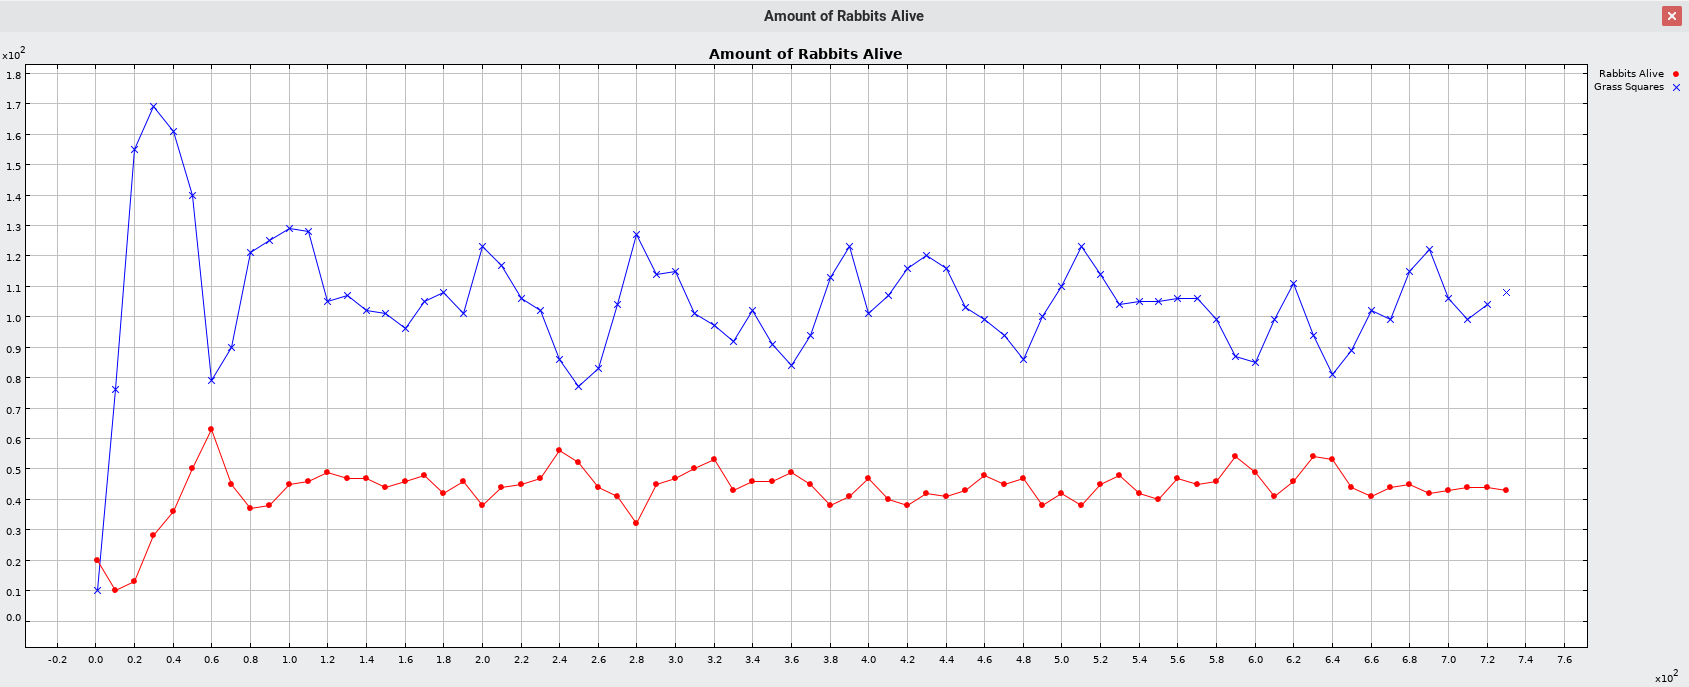
\includegraphics[width=\textwidth]{default}
	\caption{Population graph for default parameters}
	\label{fig:default}
\end{figure}

\subsection{Experiment 1: varying initial rabbits}

\subsubsection{Setting}
We tried changing the number of initial rabbits in the simulation, to see if that would have any impact on the long-term amount of rabbits. We ran simulations with 1 starting rabbit (restarting when it couldn't find food before dying), and with 300 starting rabbits.

\subsubsection{Observations}

As shown in Figure \ref{fig:exp-1}, after the first 50 turns, both simulations are stable and equivalent to the default simulation (Figure \ref{fig:default}). The only long-term difference is that, with only one rabbit, there is a high chance that it dies before finding a patch of grass; whereas with 300 it is virtually guaranteed that some of them will find enough grass to reproduce.

\begin{figure}[h]
    \centering
    \begin{subfigure}[H]{\textwidth}
        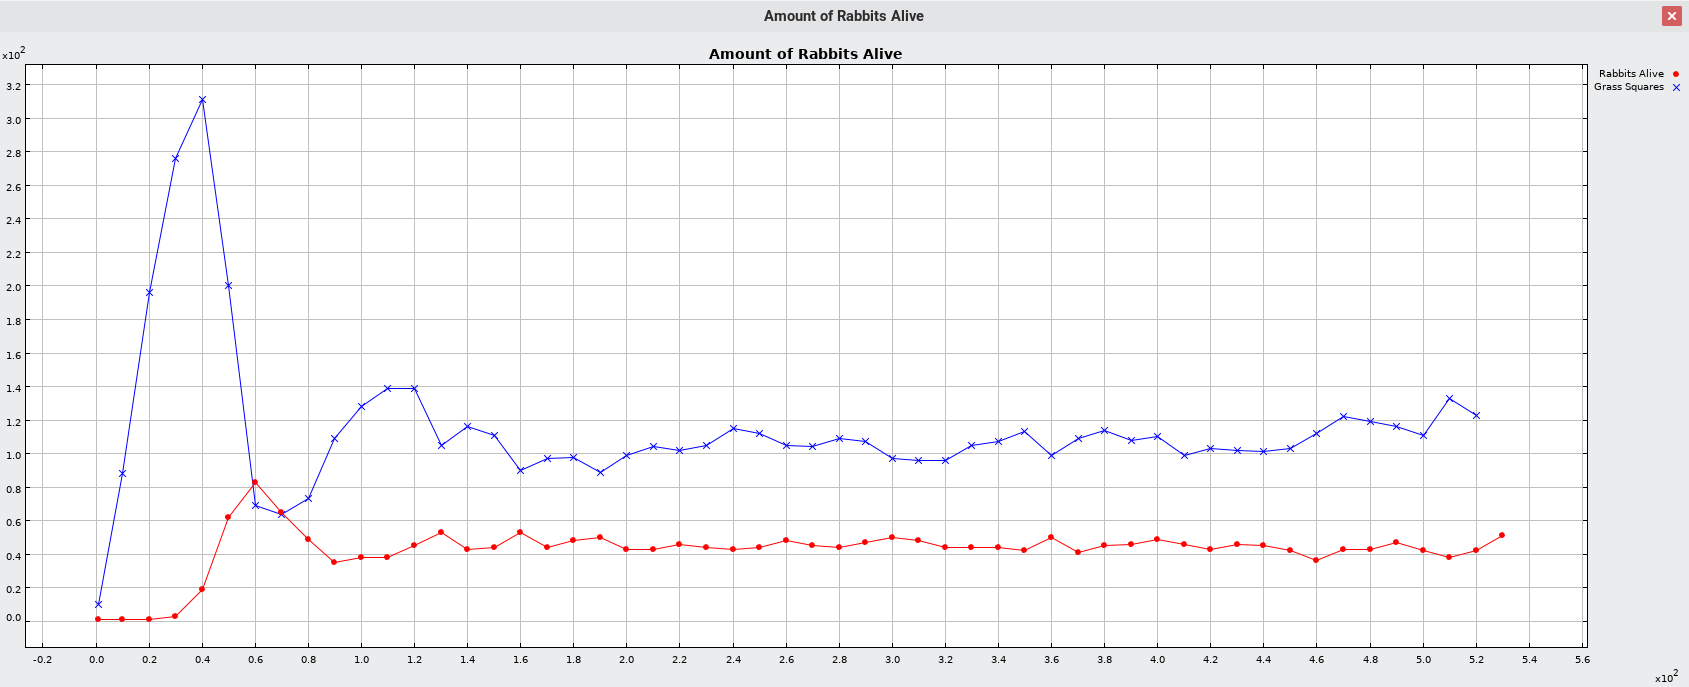
\includegraphics[width = \textwidth]{1-rabbit-default}
        \caption{Population graph for 1 starting rabbit, other values default}
        \label{fig:1-rabbit}
    \end{subfigure}
    ~
    \begin{subfigure}[H]{\textwidth}
        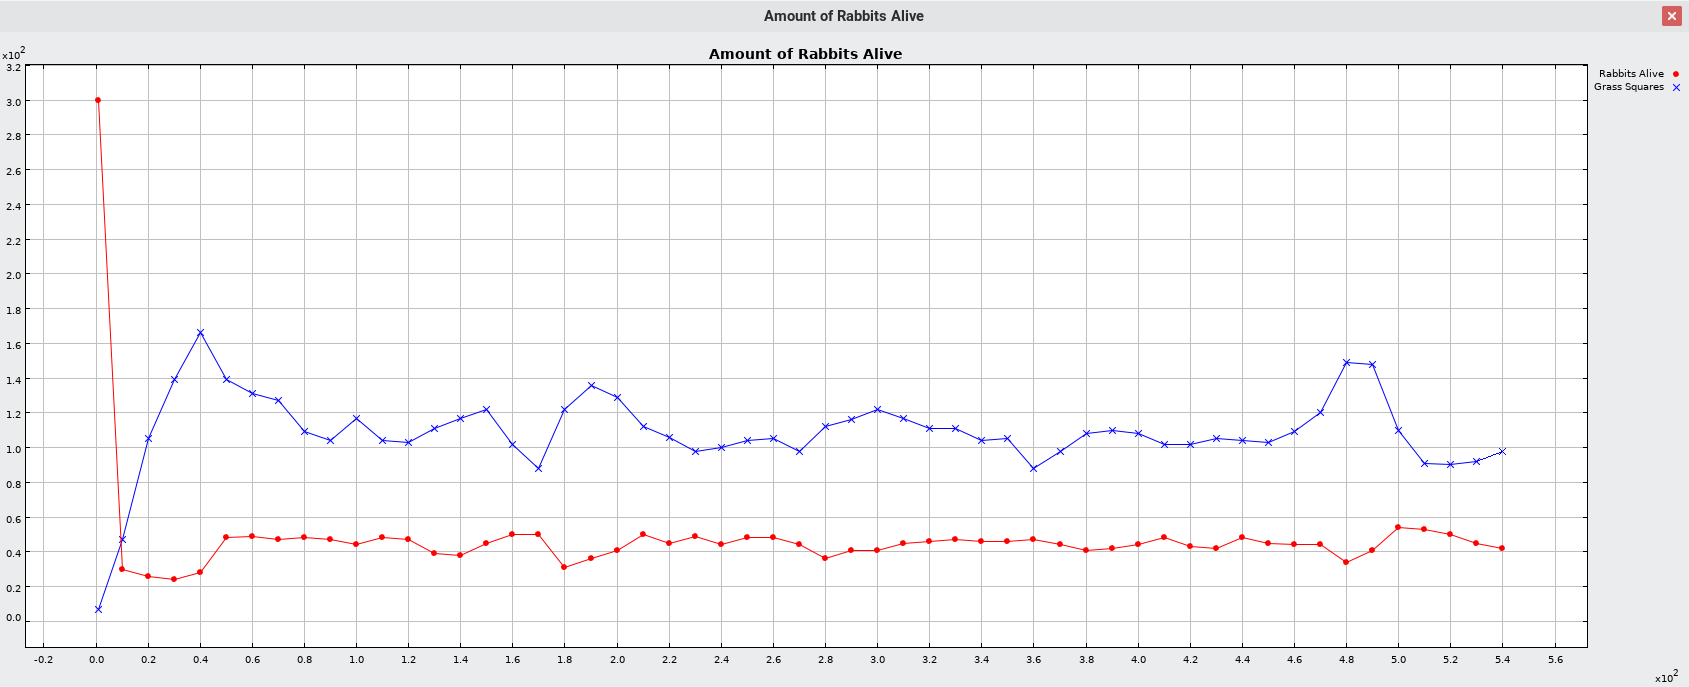
\includegraphics[width = \textwidth]{300-rabbits-default}
        \caption{Population graph for 300 starting rabbits, other values default}
        \label{fig:300-rabbits}
    \end{subfigure}
    \caption{Experiment 1}\label{fig:exp-1}
\end{figure}

\subsection{Experiment 2}

\subsubsection{Setting}

\subsubsection{Observations}
% Elaborate on the observed results %

\subsection{Experiment n}

\subsubsection{Setting}

\subsubsection{Observations}
% Elaborate on the observed results %

\end{document}